\documentclass[12pt]{article}
\usepackage[latin1]{inputenc} % Paquete para escribir en espanol.
%\usepackage[spanish]{babel} 
\usepackage[table]{xcolor} % Paquete para dar color a las letras
\usepackage{amsmath,amssymb}
\usepackage{graphicx} % Imagenes vectoriales
\usepackage{psfrag}
\usepackage{float}
\usepackage{subfigure} % Anadido por mi
\usepackage{booktabs}
\usepackage{multirow}	% Para poder unir filas en las tablas
\usepackage{setspace} % para el espacio de las filas de la tabla
\usepackage[spanish, es-tabla]{babel}
\usepackage[papersize={216mm,160mm},tmargin=5mm,bmargin=15mm,lmargin=15mm,rmargin=15mm]{geometry} 

%\textheight=10cm

\begin{document}
\pagestyle{empty}
\begin{center}
   \textit{\huge{Problema: $caso001$\\}}
	 \textit{\Large{Alumno: $Apellidos$, $Nombre$ \\}}
	 \textit{\Large{Asignatura: $Asignatura$\\}}
	 \textit{\Large{Fecha: $Fecha$\\}}	
	 \vskip 1mm
\end{center}

%\textit{Nombre}:
\vskip 4mm

% Enunciado   %%%%%%%%%%%%%%%%%%%%%%%%%%%%%%%%%%%%%%%%%%%%%%%%%%%%%%%%%%%%%%%%%%%%%%%%%%%%%%%%%%%%%%%%%%%%%%%%%%%%%
El circuito de la figura \ref{fig_circuits_1} se encuentra en regimen permanente y alimentado en D.C. Sabiendo que los valores de los elementos activos y pasivos son: $U_{AB}$=$uab$ V, $\overline{Z}_{1}$=$r1$ $\Omega$, $\overline{Z}_{2}$=$100$ $\Omega$, $\overline{Z}_{3}$=$r3$ $\Omega$, $\overline{Z}_{4}$=$1000$ $\Omega$ y $C_{5}$=$12$ $\mu F$, determinar el valor de $resultado1$:
\vskip 4mm

\begin{figure}[h!]
\centering
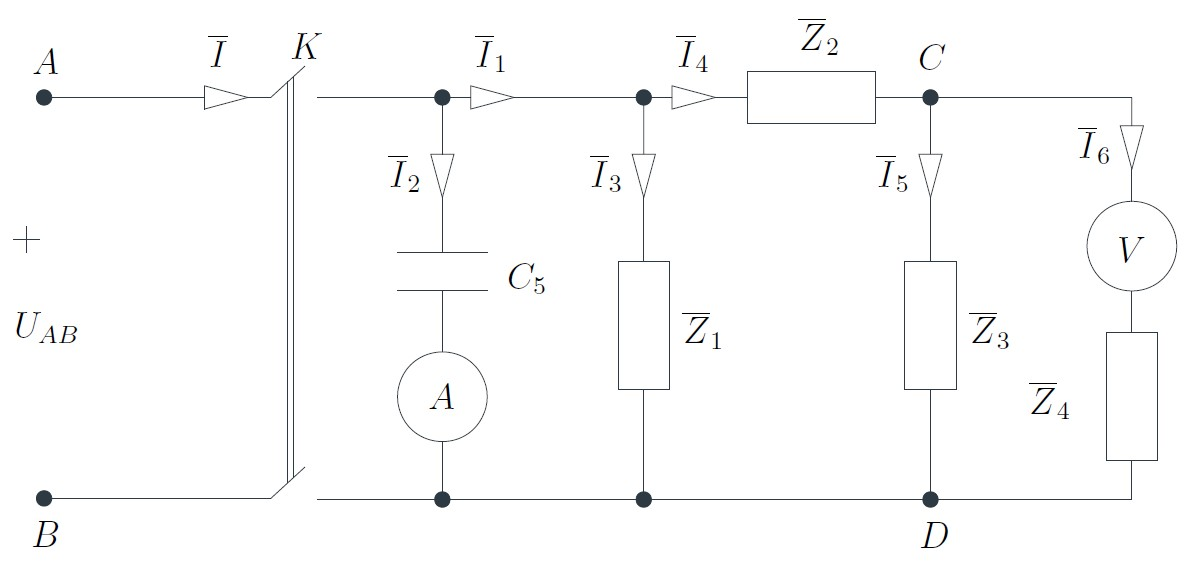
\includegraphics[width=12cm]{./caso001.png}
\caption{}\label{fig_circuits_1}
\end{figure}



\end{document}
